% This is homework.tex
% a preamble for type-setting homeworks/assignments.


%%% packages
\documentclass[11pt, a4paper, twoside]{article}

\usepackage{geometry}
\geometry{
	margin = 2cm
}
\usepackage{tikz}
	\usetikzlibrary{positioning}
\usepackage{circuitikz}
\usepackage{pgfplots}
\usepackage{lipsum}
\usepackage{fontspec}

\usepackage{amsmath}
\usepackage{amssymb}
\usepackage{enumitem}
\usepackage{graphicx}
\usepackage{fancyhdr}
\usepackage{hyperref}
\usepackage{listings}
\usepackage{multicol}
\usepackage{caption}
\usepackage{xcolor}
\usepackage{lstautogobble}
\usepackage{booktabs}
\usepackage{pdfpages}
\usepackage{fourier-orns}
\usepackage{titling}
\usepackage{lettrine}


%%% configuration
\setlength{\parindent}{0pt}
\captionsetup[figure]{width = .65\linewidth}

\renewcommand{\thefootnote}{\fnsymbol{footnote}}
\hypersetup{
	pdfborder={0 0 0},
}

\newfontface{\initials}{EB Garamond Initials}
\newfontfamily{\capitals}{Perpetua Titling MT}
\newfontfamily{\garamond}{Garamond}

\newcommand{\docfont}{\ttfamily}

\fancypagestyle{mainstyle}{
	\fancyhead[C]{}
	\fancyhead[LO, RE]{\docfont\thetitle}
	\fancyhead[LE, RO]{\docfont\thename}
	\fancyfoot[RO]{\docfont\thepage\ \floweroneright}
	\fancyfoot[LE]{\floweroneleft\ \docfont\thepage}
	\fancyfoot[LO, RE]{\docfont\thecourse}
	\fancyfoot[C]{}
	\renewcommand{\headrule}{}
	\renewcommand{\footrule}{}
}
\fancypagestyle{titlepage}{
	\fancyhead[L, C, R]{}
	\fancyfoot[RO]{\docfont\thepage\ \floweroneright}
	\fancyfoot[LE]{\floweroneleft\ \docfont\thepage}
	\fancyfoot[LO, RE]{\docfont\thecourse}
	\fancyfoot[C]{}
	\renewcommand{\headrule}{}
	\renewcommand{\footrule}{}
}

\pagestyle{mainstyle}


%%% assignment commands
\newcounter{myquestion}
\newcounter{mypart}
\makeatletter
\@addtoreset{mypart}{myquestion}
\makeatother

\newcommand{\name}[1]{\newcommand{\thename}{#1}}
\newcommand{\roll}[1]{\newcommand{\theroll}{#1}}
\newcommand{\program}[1]{\newcommand{\theprogram}{#1}}
\newcommand{\course}[1]{\newcommand{\thecourse}{#1}}
\renewcommand{\date}[1]{\newcommand{\thedate}{#1}}
\renewcommand{\title}[2]{
	\newcommand{\thetitle}{#1#2}
	\newcommand{\thefancytitle}{
		{\fontsize{60}{68}\selectfont\initials#1}{\huge\scshape#2}
	}
}

\newcommand{\myheader}[1]{
	\noindent\bigskip
	\begin{center}
		{\Large\docfont\bfseries #1}
	\end{center}
	\vspace{-.25\baselineskip}
}
\NewDocumentCommand{\myquestion}{ o m }{
	\IfNoValueTF{#1}{
		\stepcounter{myquestion}
		\par\vspace{\baselineskip}
		{\docfont\bfseries Question \themyquestion:} #2 \par
	}{%
		\stepcounter{myquestion}
		\setcounter{myquestion}{#1}
		\par\vspace{\baselineskip}
		{\docfont\bfseries Question #1:} #2 \par
	}
}
\newcommand{\mypart}[1]{
	\stepcounter{mypart}
	\par\vspace{.5\baselineskip}
	{\docfont\bfseries Part (\roman{mypart}):} {#1} \par
}
\newcommand{\mysol}{\par{\docfont Solution. }}
\NewDocumentCommand{\mynote}{ o m }{
	\IfNoValueTF{#1}{
		\begin{center}
			\fbox{\parbox{.8\linewidth}{
				{\docfont Note} \\[.25\baselineskip] {\small #2}
			}}
		\end{center}
	}{
		\begin{center}
			\fbox{\parbox{.8\linewidth}{
				{\docfont Note} \hfill {\docfont\itshape (#1)} \hfill \\[.25\baselineskip] {\small #2}
			}}
		\end{center}
	}
}

\newcommand{\printheadclean}{
	\thispagestyle{titlepage}
	\renewcommand{\docfont}{\normalfont}
	\begin{center}
		\begin{tikzpicture}[overlay]
			\foreach \i in {-3, -1, 1, 3} {
				\draw[line width = 1.5pt] (-.5\linewidth, .175*\i) -- (.5\linewidth, .175*\i);
			}
			\node[fill = white, text = black, draw = white] at (0, 0) {\huge\bfseries\capitals\thetitle};
		\end{tikzpicture}
	\end{center} \par \vspace{\baselineskip} \noindent
	Name: {\bfseries\thename} (\theroll) \hfill Submitted on \thedate \hfill \\
	Program: \theprogram \\
	Course: \thecourse \\
	\rule{\linewidth}{1.5pt}
}
\newcommand{\printheadbox}{
	\thispagestyle{titlepage}
	\renewcommand{\docfont}{\ttfamily}
	\fbox{
		\parbox{\linewidth}{{
			\ttfamily
			\bigskip
			{\bfseries\thename} (\theroll) \hfill \bfseries\thetitle \hfill \\
			\normalfont\ttfamily\theprogram \hfill \thecourse \hfill
			\begin{center}
				Submitted\ \thedate
			\end{center}
		}
	}}
}
\newcommand{\printheadfancy}{
	\renewcommand{\docfont}{\garamond}
	\thispagestyle{titlepage}
	\begin{center} 
		{\Huge\thefancytitle}
	\end{center} 
	\vspace{2\baselineskip}
	{
		\garamond\Large
		{\bfseries\thename} \hfill {\large Submitted \thedate} \hfill \\[3pt]
		(\theroll) \hfill {\bfseries\thecourse} \\[8pt]
		{\itshape\theprogram}
	}
	\begin{center}
		{\huge\decoone}
	\end{center}
}


%%% computer science
\lstset{
	language = Python,
	tabsize = 4,
	basicstyle = \ttfamily\small,
	breaklines = true,
	autogobble = true,
	numbers = left,
	firstnumber = last,
	numberstyle = \tiny\color{black!70},
	commentstyle = \color{black!70},
	keywordstyle = ,
	xrightmargin = .1\linewidth,
	aboveskip = .5\baselineskip,
	belowskip = \baselineskip,
	showstringspaces = false
}
\newcommand{\mylanguage}[1]{
	\lstset{language = #1},
}

\lstnewenvironment{lstoutput}
{
	\texttt{\#\#\# Output:}
	\lstset{
		basicstyle = \ttfamily\small,
		breaklines = true,
		autogobble = true,
		tabsize = 4,
		numbers = none,
		xleftmargin = .05\linewidth,
		xrightmargin = .15\linewidth,
		frame = single
	}
}
{
}

%%% mathematics generic
\newcommand{\mytheorem}[1]{
	\vspace{.5\baselineskip}
	{\docfont\bfseries Theorem.} {\itshape #1} \par
}

\newcommand{\myclaim}[1]{
	\vspace{.5\baselineskip}
	{\docfont\bfseries Claim.} {\itshape #1} \par
}

\newcommand{\myproof}[1]{
	\vspace{.5\baselineskip}
	{\docfont\itshape Proof.} #1 \hfill $\blacksquare$
}


\let\originalforall\forall
\let\originalexists\exists
\renewcommand{\forall}{\ \originalforall\ }
\renewcommand{\exists}{\ \originalexists\ }

\newcommand{\inv}{^{-1}}
\newcommand{\lcm}[1]{\text{lcm}(#1)}
\newcommand{\bb}[1]{\mathbb{#1}}
\newcommand{\ri}[1]{\mathcal{#1}}
\newcommand{\der}[1]{\, \text d#1}
\newcommand{\derfrac}[2]{\frac{\der{#1}}{\der{#2}}}


%%% group theory
\ExplSyntaxOn
\NewDocumentCommand{\cycle}{ O{\;} m }
{
	(
	\alec_cycle:nn { #1 } { #2 }
	)
}
\seq_new:N \l_alec_cycle_seq
\cs_new_protected:Npn \alec_cycle:nn #1 #2
{
	\seq_set_split:Nnn \l_alec_cycle_seq { , } { #2 }
	\seq_use:Nn \l_alec_cycle_seq { #1 }
}
\ExplSyntaxOff

\ExplSyntaxOn
\NewDocumentCommand{\seplist}{ O{\ } m} {
	\seq_set_from_clist:Nn \l_tmpa_seq {#2}
	\seq_use:Nn \l_tmpa_seq { #1 }
}
\ExplSyntaxOff

\newcommand{\tsymmetry}[5]{
	\begin{tikzpicture}[scale = .5]
		\draw[black!50, line width = 2pt] (-1.5, -1.5) -- (1.5, -1.5) -- (0, 1.5) -- cycle;
		\node[fill opacity = 0, draw opacity = 0, text opacity = 1, text = black!50] at (-1.85, -1.85) {\bfseries1};
		\node[fill opacity = 0, draw opacity = 0, text opacity = 1, text = black!50] at (1.85, -1.85) {\bfseries2};
		\node[fill opacity = 0, draw opacity = 0, text opacity = 1, text = black!50] at (0, 1.95) {\bfseries3};
		\draw[->, line width = 2pt] (2, 0) -- (4, 0);
		\draw[line width = 2pt] (4.5, -1.5) -- (7.5, -1.5) -- (6, 1.5) -- cycle;
		\node[fill opacity = 0, draw opacity = 0, text opacity = 1, text = black] at (4.15, -1.85) {\bfseries#1};
		\node[fill opacity = 0, draw opacity = 0, text opacity = 1, text = black] at (7.85, -1.85) {\bfseries#2};
		\node[fill opacity = 0, draw opacity = 0, text opacity = 1, text = black] at (6, 1.95) {\bfseries#3};
		\node at (3, -3) {#4 | In cycle form: #5};
	\end{tikzpicture}
}

\newcommand{\class}[1]{\left\langle #1 \right\rangle}
\newcommand{\aut}[1]{\text{Aut}(#1)}
\newcommand{\inn}[1]{\text{Inn}(#1)}
\renewcommand{\ker}[1]{\text{Ker}#1}


%%% riemann integration
\newcommand{\uppers}[2]{\text{U}(#1, #2)}
\newcommand{\lowers}[2]{\text{L}(#1, #2)}
\newcommand{\reis}[2]{\text{S}(#1, #2)}
\newcommand{\upperi}[1]{\text{U}(#1)}
\newcommand{\loweri}[1]{\text{L}(#1)}
\newcommand{\mesh}[1]{\text{mesh}(#1)}


%%% other generic commands
\newcommand{\insertitem}[1]{\item #1}
\NewDocumentCommand{\mylist}{>{\SplitList{;;;}}m}
{
	\begin{enumerate}[itemsep = 0pt, topsep = 0pt, parsep = 0pt, partopsep = 0pt, leftmargin = *]
		\ProcessList{#1}{\insertitem}	
	\end{enumerate}
}